\section{Import to InteliJ IDEA}
\label{sec:imp_idea}

\begin{figure}[H]
	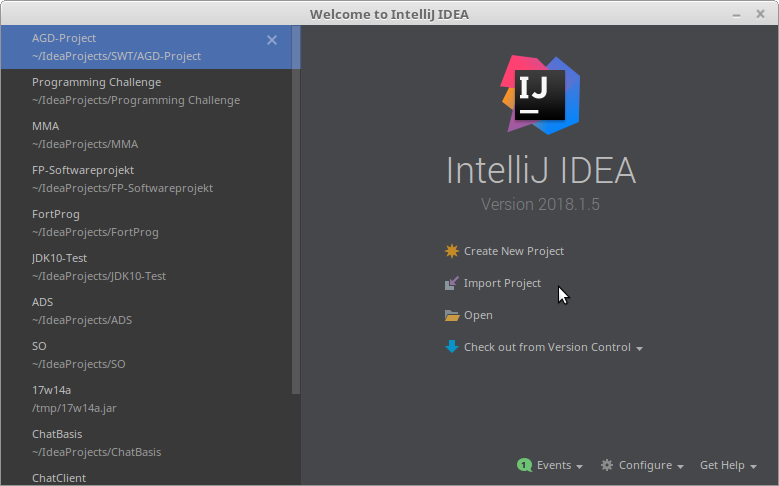
\includegraphics[width=\textwidth]{setup-parts/pictures/idea-import-1a.png}
	\caption[width=\textwidth/2]{If you start here click on \textit{"Import Project"}}
\end{figure}
\begin{figure}[H]
	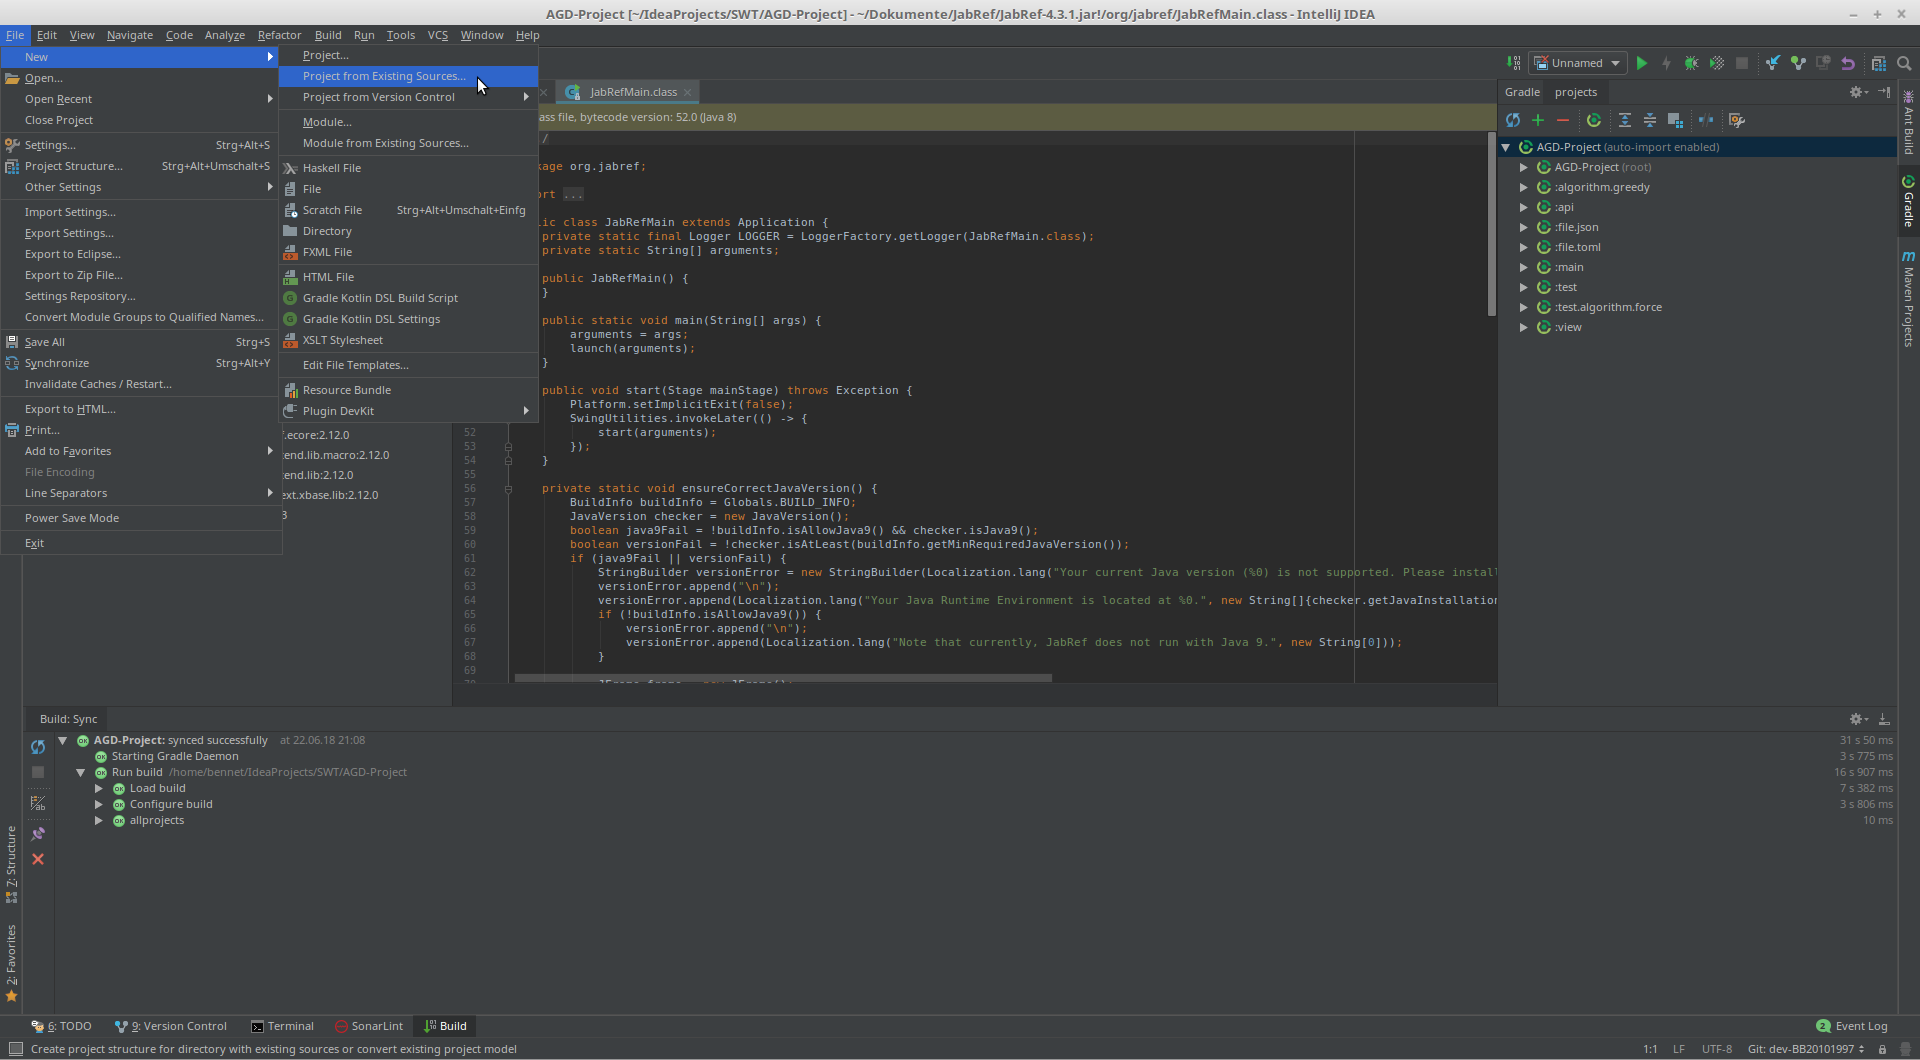
\includegraphics[width=\textwidth]{setup-parts/pictures/idea-import-1b.png}
	\caption[width=\textwidth/2]{If you start here click on \textit{"File $\rightarrow$ New $\rightarrow$ Project from Existing Source"}}
\end{figure}

\begin{figure}[H]
	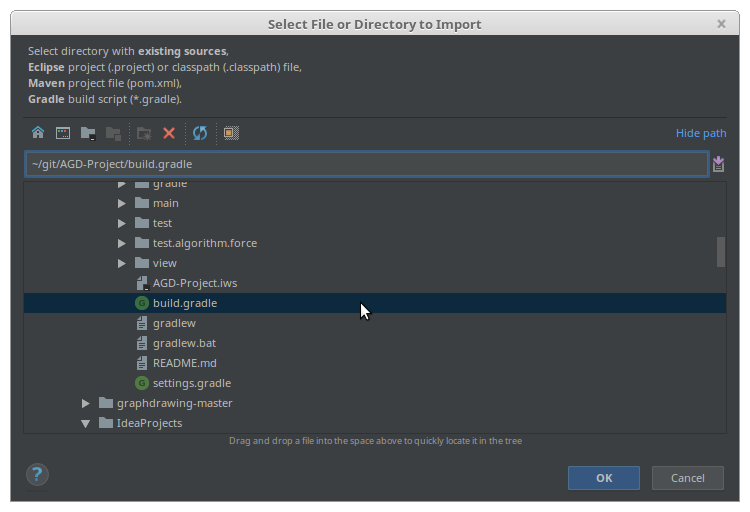
\includegraphics[width=\textwidth]{setup-parts/pictures/idea-import-2.png}
	\caption{Now select either \textit{"build.gradle"} or \textit{"settings.gradle"} in the project root.}
\end{figure}

\begin{figure}[H]
	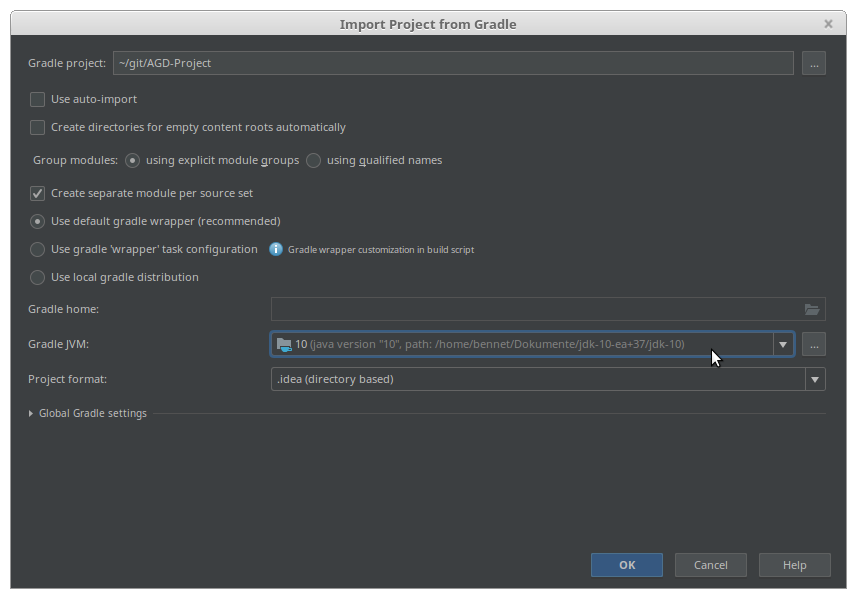
\includegraphics[width=\textwidth]{setup-parts/pictures/idea-import-3.png}
	\caption{Make sure Gradle JVM is at least Java 10, then click "OK" and you are done.}
\end{figure}